\documentclass[tikz,border=8pt]{standalone}
\usetikzlibrary{arrows.meta,calc,angles,quotes}
\definecolor{ink}{HTML}{17324D}
\definecolor{blue}{HTML}{1877B8}
\definecolor{orange}{HTML}{D97706}
\definecolor{green}{HTML}{16856B}
\definecolor{red}{HTML}{C24156}
\begin{document}
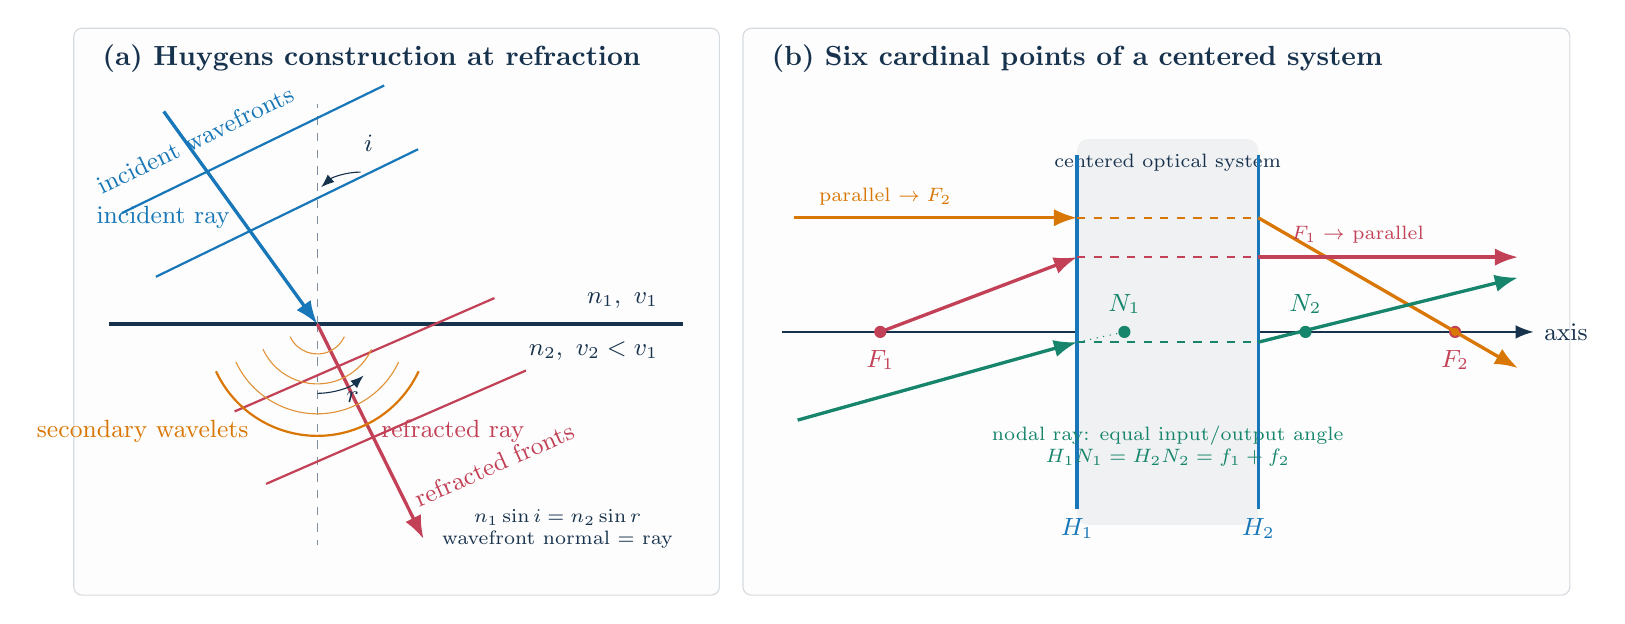
\begin{tikzpicture}[font=\small,>=Latex]
\tikzset{panel/.style={draw=ink!18,rounded corners=3pt,fill=ink!1}}

\node[panel,minimum width=8.2cm,minimum height=7.2cm,anchor=south west] at (0,0) {};
\node[font=\bfseries,ink,anchor=west] at (.25,6.82) {(a) Huygens construction at refraction};
\draw[very thick,ink] (.45,3.45)--(7.75,3.45);
\node[ink,anchor=south east] at (7.55,3.52) {$n_1,\ v_1$};
\node[ink,anchor=north east] at (7.55,3.35) {$n_2,\ v_2<v_1$};
\coordinate (A) at (3.1,3.45);
\draw[dashed,ink!55] (A)--(3.1,6.25);
\draw[dashed,ink!55] (A)--(3.1,.65);
\draw[->,blue,very thick] (1.15,6.15)--(A) node[midway,left] {incident ray};
\draw[->,red,very thick] (A)--(4.45,.72) node[midway,right] {refracted ray};
\draw[blue,thick] (.62,4.86)--(3.95,6.48);
\draw[blue,thick] (1.05,4.05)--(4.38,5.67);
\node[blue,anchor=south,rotate=26] at (1.65,5.58) {incident wavefronts};
\draw[red,thick] (2.05,2.34)--(5.35,3.78);
\draw[red,thick] (2.45,1.42)--(5.75,2.86);
\node[red,anchor=north,rotate=24] at (5.25,1.88) {refracted fronts};
\foreach \r in {.38,.76,1.14}{
  \draw[orange!80,thin] (A) ++(205:\r) arc[start angle=205,end angle=335,radius=\r];
}
\draw[orange,thick] (A) ++(205:1.42) arc[start angle=205,end angle=335,radius=1.42];
\node[orange,anchor=north east] at (2.35,2.35) {secondary wavelets};
\draw[->,ink] (3.65,5.38) arc[start angle=90,end angle=132,radius=.75];
\node[ink] at (3.75,5.75) {$i$};
\draw[->,ink] (3.1,2.57) arc[start angle=-90,end angle=-48,radius=.88];
\node[ink] at (3.55,2.52) {$r$};
\node[align=center,font=\scriptsize,ink] at (6.15,.85)
  {$n_1\sin i=n_2\sin r$\\wavefront normal $=$ ray};

\node[panel,minimum width=10.5cm,minimum height=7.2cm,anchor=south west] at (8.5,0) {};
\node[font=\bfseries,ink,anchor=west] at (8.75,6.82) {(b) Six cardinal points of a centered system};
\begin{scope}[shift={(9.0,3.35)}]
  \draw[->,ink,thick] (0,0)--(9.55,0) node[right] {axis};
  \fill[ink!7,rounded corners=4pt] (3.75,-2.45) rectangle (6.05,2.45);
  \node[ink,font=\scriptsize] at (4.9,2.15) {centered optical system};
  \draw[blue,very thick] (3.75,-2.25)--(3.75,2.25);
  \draw[blue,very thick] (6.05,-2.25)--(6.05,2.25);
  \node[blue,below] at (3.75,-2.25) {$H_1$};
  \node[blue,below] at (6.05,-2.25) {$H_2$};
  \fill[red] (1.25,0) circle (2.2pt) node[below=3pt] {$F_1$};
  \fill[red] (8.55,0) circle (2.2pt) node[below=3pt] {$F_2$};
  \fill[green] (4.35,0) circle (2.2pt) node[above=3pt] {$N_1$};
  \fill[green] (6.65,0) circle (2.2pt) node[above=3pt] {$N_2$};

  % Parallel ray to rear focus.
  \draw[->,orange,very thick] (.15,1.45)--(3.75,1.45);
  \draw[orange,dashed,thick] (3.75,1.45)--(6.05,1.45);
  \draw[->,orange,very thick] (6.05,1.45)--(9.35,-.46);
  \fill[orange] (8.55,0) circle (1.5pt);

  % Front-focus ray to parallel output.
  \draw[->,red,very thick] (1.25,0)--(3.75,.95);
  \draw[red,dashed,thick] (3.75,.95)--(6.05,.95);
  \draw[->,red,very thick] (6.05,.95)--(9.35,.95);

  % Nodal ray, same physical angle in and out.
  \coordinate (P1) at (3.75,-.13);
  \coordinate (P2) at (6.05,-.13);
  \draw[->,green,very thick] (.20,-1.12)--(P1);
  \draw[green,dashed,thick] (P1)--(P2);
  \draw[->,green,very thick] (P2)--(9.35,.69);
  \draw[green,dotted] (P1)--(4.35,0);
  \draw[green,dotted] (P2)--(6.65,0);

  \node[orange,font=\scriptsize,anchor=south west] at (.35,1.48) {parallel $\to F_2$};
  \node[red,font=\scriptsize,anchor=south west] at (6.35,1.0) {$F_1\to$ parallel};
  \node[green,font=\scriptsize,align=center] at (4.9,-1.45)
    {nodal ray: equal input/output angle\\$H_1N_1=H_2N_2=f_1+f_2$};
\end{scope}
\end{tikzpicture}
\end{document}
